\documentclass[tikz,12pt]{standalone}

\usepackage{tikz}

\renewcommand*{\familydefault}{\sfdefault}
    
\begin{document}

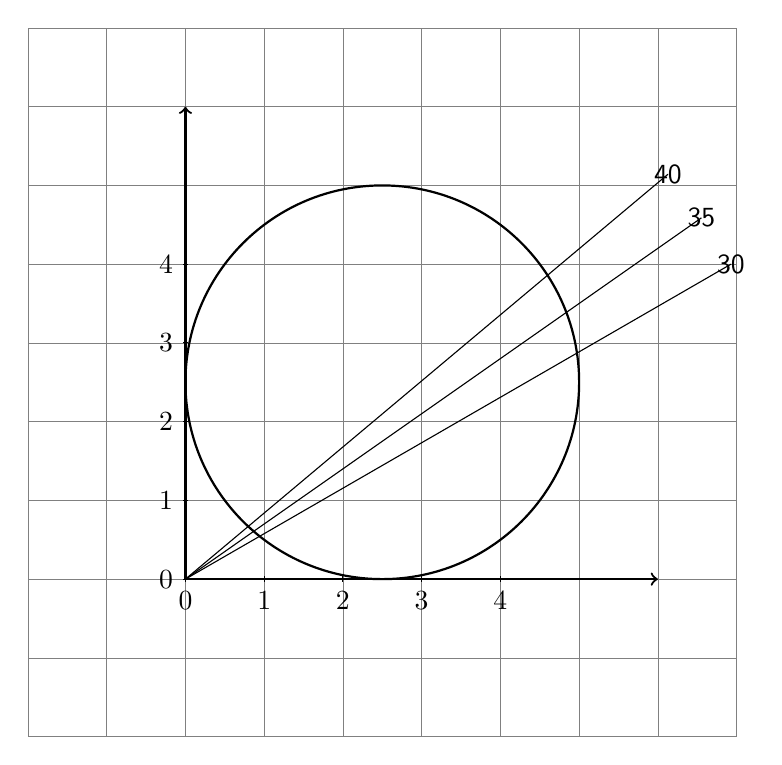
\begin{tikzpicture}
	\draw[step=1cm,gray,very thin] (-2,-2) grid (7,7);

	\draw [thick, ->] (0,0) -- ++ (0,6cm);
	\draw [thick, ->] (0,0) -- ++ (6cm, 0);
	\draw [thick] (2.5,2.5) circle (2.5cm); 

	\foreach \x in {0,1,2,3,4}
    	\draw (\x cm,1pt) -- (\x cm,-1pt) node[anchor=north] {$\x$};
	\foreach \y in {0,1,2,3,4}
    	\draw (1pt,\y cm) -- (-1pt,\y cm) node[anchor=east] {$\y$};

	\draw (0,0) -- (30:8cm) node {30};
	\draw (0,0) -- (35:8cm) node {35};
	\draw (0,0) -- (40:8cm) node {40};

\end{tikzpicture}
  
\end{document}